\chapter{Static One Body Problem}\label{ch:chapter2}


The metric given in (\ref{eq:finalmetricpn}) is the general form of the Post-Newtonian metric, nevertheless a even more general metric is desired. The called Parametrized Post - Newtonian (PPN) is written in terms of a set of parameters can describe more than one theory. \\

The final purpose of this Chapter is to construct and determine the equation of motions for one static body system. The field produced by this body must meet with the conditions of a weak field, introduced in the Chapter \ref{ch: firstchapter}. For the construction of these equations, the PPN metric is used.\\

\section{Parametrized Metric}

Let consider first the Schwarzschild metric. This is the solution of the Einstein field equations outside a spherically symmetric and static body, meaning the solution is independent of the time and invariant under the reflection $t \rightarrow -t$,
\begin{equation}
\label{eq: Schwarzschild metric}
ds^2 = -\left(1-\frac{2m}{r}\right) c^2 dt^2 + \left(1-\frac{2m}{r}\right)^{-1} dr^2 + r^2 (d\theta^2 +\sin^2\theta d\phi^2),
\end{equation}
in geometric units, where $G = 1$, $c = 1$, and the mass is
\begin{equation}
m=\frac{GM}{c^{\,2}}.
\end{equation}



All the results until now are based on the use of the Standard Post-Newtonian gauge, introduced in Chapter \ref{ch: firstchapter} in equation (\ref{eq: standardgauge}),

\begin{equation}
\partial_\mu (\sqrt{-g}g^{\mu\nu})=0  \rightarrow g^{\mu\nu}\Gamma_{\mu\nu}^{\alpha}=0.
\end{equation}
These conditions imply the use of a coordinate system that meets the following condition,
\begin{align}
\Box z  ^\beta =0\\
g^{\alpha\beta} \nabla_\alpha\nabla_\beta z  ^\beta = 0.
\end{align}
For a scalar field, $\nabla_\beta z  ^\beta = \partial_\beta z  ^\beta$, and then
\begin{align}
\label{eq: backto}
g^{\alpha\beta} \nabla_\alpha \partial_\beta z  ^\beta = \nabla_\alpha (g^{\alpha\beta}\partial_\beta z  ^\beta).
\end{align}
A covariant derivative is defined as
\begin{align*}
\nabla_\mu V^\mu = \partial_\mu V^\mu + \Gamma^{\mu}_{\mu\alpha}V^\alpha, 
\end{align*}
where (See \cite{Weinberg})
\begin{align*}
\Gamma^{\mu}_{\mu\alpha} &= \frac{1}{2}g^{\mu\kappa}\left(\partial_\alpha g_{\kappa\mu}+\partial_\mu g_{\kappa\alpha}- \partial_\kappa g_{\mu\alpha}\right)\\
&=\frac{1}{2}g^{\mu\kappa}\left(\partial_\alpha g_{\kappa\mu}\right)\\
&=\frac{1}{2}\partial_\alpha(ln g)\\
&=\frac{1}{\sqrt{g}}\partial_\alpha(\sqrt{g}).
\end{align*}

Replacing this expression into $\nabla_\mu V^\mu$,
\begin{align*}
\nabla_\mu V^\mu = \partial_\mu V^\mu +\frac{1}{\sqrt{-g}}\partial_\alpha(\sqrt{-g})V^\alpha = \frac{1}{\sqrt{-g}}\partial_\alpha(\sqrt{-g}V^\alpha),
\end{align*}

replacing these expressions into (\ref{eq: backto})
\begin{align}
\nabla_\alpha (g^{\alpha\beta}\partial_\beta z  ^\beta) =  \frac{1}{\sqrt{-g}} \partial_\alpha(\sqrt{-g}g^{\alpha\beta}\partial_\beta z^\beta) = 0.
\end{align}

For $z  ^\beta = (ct,x,y,z)$,
\begin{align}
 \partial_\alpha(\sqrt{-g}g^{\alpha\beta}) = 0.
\end{align}

These type of coordinates are named quasi-harmonic, ``quasi'' because there are not exactly inertial coordinates due to the fact that it defines the position of a particle around a gravitational source.\\

The Schwarzschild metric given in (\ref{eq: Schwarzschild metric}) can be rewritten in terms of harmonic coordinates. Making a linear transformation of the $r$ component, where $r_h$ means for harmonic,
\begin{equation*}
	r = r_h+m,
\end{equation*}
We obtain,
\begin{equation*}
	ds^2 = -\left(\frac{1-\frac{m}{r_h}}{1+\frac{m}{r_h}}\right) c^2 dt^2 + \left(\frac{1+\frac{m}{r_h}}{1-\frac{m}{r_h}}\right) dr_h^2 + r_h ^2 \left(1+\frac{m}{r_h}\right)^{2} (d\theta^2 + \sin^2\theta d\phi^2).
\end{equation*}
In cartesian coordinates, this is
\begin{equation}
	ds^2 = -\left(\frac{1-\frac{m}{r_h}}{1+\frac{m}{r_h}}\right) c^2 dt^2 + \left(1+\frac{m}{r_h}\right)^{2} \left[\delta_{ij}+\frac{\left(\frac{m}{r_h}\right)^2}{1-\left(\frac{m}{r_h}\right)^2}\frac{x_ix_j}{r_h^2}\right]dx^idx^j.
\end{equation}

Making the approximation $\epsilon^2 \sim \frac{m}{r_h}<<1$, 
%entre mas lejos del cuerpo esférico, mas débiles son los efectos gravitacionales. (aproximación post newtonian) 
\begin{align}
 \begin{split}
ds^2 =& -\left[1-\frac{2m}{r_h}+\frac{2m^2}{r_h^2}+\mathcal{O}(\epsilon^6)\right]c^2 dt^2 \\
&+ \left[\delta_{ij}+\frac{2m}{r_h}\delta_{ij}+\frac{m^2}{r_h^2}\left(\delta_{ij}+\frac{x_ix_j}{r_h^2}\right)+\mathcal{O}(\epsilon^6)\right]dx^idx^j.
\end{split}
\end{align}

As it was mentioned above, the metric given below is rewritten as a PPN metric \cite{Brumberg},
\begin{subequations}
\label{eq:gmetricppn}
\begin{align}
&g_{00} =  -\left[1-2\kappa\frac{m}{r_h}+2(\beta-\alpha)\frac{m^2}{r_h^2}+\mathcal{O}(\epsilon^6)\right]\\
&g_{0j} =  0\\
&g_{ij} = \left[\delta_{ij}+\frac{2m}{r_h}\left[(\gamma-\alpha)\delta_{ij}+\alpha\frac{x_ix_j}{r_h^2}\right]+\mathcal{O}(\epsilon^4)\right],
\end{align}
\end{subequations}

where \cite{GravityPoisson},
\begin{itemize}
\item $\kappa$: Measures the newtonian contribution
\item $\beta$ y $\alpha$: Measures the non-linear contribution
\item $\gamma$:  Measures the curvature because of the body that produces the gravitational field.
\end{itemize}


The action describing a test particle of mass $m_0$ \cite{GravityPoisson} is 
\begin{align*}
\mathcal{S} = -\int_{t_1}^{t_2}Ldt  = -m_0c^2\int_{t_1}^{t_2}\frac{d\tau}{dt}dt,
\end{align*}
where $\tau$ is the proper time of the particle and $t$ is the time of an asymptotic observer.
\begin{align*}
&ds^2=-c^2d\tau^2 = g_{\mu\nu}dx^\mu dx^\nu\\
&\left(\frac{d\tau}{dt}\right)^2 = -g_{\mu\nu}\frac{\dot{x}^\mu\dot{x}^\nu}{c^2}.
\end{align*}

The metric tensor $g_{\mu\nu}$ is
\begin{subequations}
\label{eq:metricgeneral}
\begin{align}
		&g_{00} = -1+ ^{(2)}\hspace{-0.1cm}h_{00}+ ^{(4)}\hspace{-0.1cm}h_{00}+\mathcal{O}(\epsilon^6)\\
		&g_{0j} = \hspace{-0.1cm}^{(3)}\hspace{-0.05cm}h_{0j}+ \mathcal{O}(\epsilon^5) \\
		&g_{jk} = \delta_{jk}+^{(2)}\hspace{-0.1cm}h_{jk}+\mathcal{O}(\epsilon^4).
\end{align}
\end{subequations}
Replacing above,
\begin{align}
\label{eq:dtaudt}
\left(\frac{d\tau}{dt}\right)^2&=1-^{(2)}h_{00}-^{(4)}h_{00}-2^{(3)}h_{0j}\frac{\dot{x}^{0}\dot{x}^{j}}{c^2}-^{(2)}h_{ij}\frac{\dot{x}^{i}\dot{x}^{j}}{c^2}-\frac{\dot{\mathbf{x}}^2}{c^2}.
\end{align}

\section{Lagrangian and equations of motion}
The Lagrangian for the test particle is
\begin{align*}
L = -m_0c^2\left(\frac{d\tau}{dt}-1\right),
\end{align*}
where $\frac{d\tau}{dt} = \sqrt{\left(\frac{d\tau}{dt}\right)^2}$ is obtained from the equation (\ref{eq:dtaudt}) and considering the expansion $(1+x)^n$ when $x << 1$,
\begin{align}
\label{eq:firstlagrangian}
\begin{split}
L &= \frac{1}{2} m_0 \dot{\mathbf{x}}^2 + \frac{1}{2}m_0c^{2(2)}h_{00} + \frac{1}{8} m_0 \frac{(\dot{\mathbf{x}}^{2})^2}{c^2}  + \frac{1}{2} m_0c^{2(4)}h_{00} + m_0 c^{(3)}h_{0j} \dot{x}^j \\
&+ \frac{1}{2} m_0 ^{(2)}h_{ij}\dot{x}^{i} \dot{x}^{j} + \frac{1}{8} m_0 c^{2}\left(^{(2)}h_{00} \right)^{2} + \frac{1}{4} m_0^{(2)}h_{00} \dot{\mathbf{x}}^2 + \mathcal{O}(\epsilon^3).
\end{split} 
\end{align}

The associated equations of motion can be extracted in the usual way, with the Euler-Lagrange equations.
\begin{align*}
	&\frac{d}{dt}\left(\frac{\partial L}{\partial \dot{x}^j}\right) = \frac{\partial L}{\partial x^j},
	\end{align*}
	\begin{align}
	\begin{split}
	\label{eq:equationsofmotion}
	\ddot{x}^j &= \frac{1}{2}c^2\partial_{j}^{(2)}h_{00}+\frac{1}{2}c^2\partial_{j}^{(4)}h_{00}-\frac{1}{2}c^{2(2)}h_{jk}\partial_{k}^{(2)}h_{00}-c^2 \partial_0^{(3)}h_{0j} -\frac{1}{2}c\dot{x}^j\partial_0^{(2)}h_{00} \\
	&-c\dot{x}^k\partial_0^{(2)}h_{jk}-c\left(\partial_k^{(3)}h_{0j}-\partial_j^{(3)}h_{0k}\right)\dot{x}^k
	-\dot{x}^j\dot{x}^k\partial_k^{(2)}h_{00} \\
	&- \left(\partial_k^{(2)}h_{jl}-\frac{1}{2}\partial_j^{(2)}h_{kl}\right)\dot{x}^k\dot{x}^l + \mathcal{O}(\epsilon^3).
	\end{split}
	\end{align}


The Lagrangian in (\ref{eq:firstlagrangian}) and the equations of motion given in (\ref{eq:equationsofmotion}) can be rewritten in terms of the components of the tensor $h_{\mu\nu}$ given in (\ref{eq:gmetricppn}), and (\ref{eq:metricgeneral}) (See \cite{Brumberg} with $\kappa = 1$).\\

The Lagrangian
\begin{align}
\begin{split}
L &= \frac{1}{2} m_0 \dot{\mathbf{x}}^2 +  GM \kappa \frac{m_0}{r}+ \frac{1}{8} m_0 \frac{(\dot{\mathbf{x}}^{2})^2}{c^2}  \\
&+ \frac{m m_0}{r}\left[\left(\gamma + \frac{1}{2}\kappa-\alpha \right) \dot{\mathbf{x}}^2+\left(\alpha + \frac{1}{2}\kappa^2-\beta \right)\frac{GM}{r}+\alpha \frac{\left(\mathbf{x}\cdot\mathbf{\dot{x}}\right)}{r^2}\right]+\mathcal{O}(\epsilon^4)
\end{split}
\end{align}

and the equations of motion
\begin{align*}
\begin{split}
\ddot{x}^j + \frac{\kappa GM}{r^3}x^j &= \frac{m}{r^3}\left[2(\beta + \kappa \gamma - \alpha)\frac{GM}{r}-(\gamma+\alpha)\dot{x}_k\dot{x}^k+ 3\alpha\frac{\left(x_k\dot{x}^k\right)^2}{r^2}\right]x^j\\
&+\frac{m}{r^3}\left[2(\kappa+\gamma - \alpha)x_k\dot{x}^k\right]\dot{x}^j+\mathcal{O}(\epsilon^3).
\end{split}
\end{align*}

In vector notation, these are
\begin{align}
\begin{split}
\label{eq: equationofmotion}
\mathbf{\ddot{x}^} + \frac{\kappa GM}{r^3}\mathbf{x} &= \frac{m}{r^3}\left[2(\beta + \kappa \gamma - \alpha)\frac{GM}{r}-(\gamma+\alpha)\mathbf{\dot{x}}^2+ 3\alpha\frac{\left(\mathbf{x} \cdot \mathbf{\dot{x}}\right)^2}{r^2}\right]\mathbf{x}\\
&+\frac{m}{r^3}\left[2(\kappa+\gamma - \alpha)\mathbf{x}\cdot\mathbf{\dot{x}}\right]\mathbf{\dot{x}}+\mathcal{O}(\epsilon^3).
\end{split}
\end{align}

\section{Conserved quantities}

To determine the conserved quantities, transform to polar coordinates
\begin{align*}
&\mathbf{x} =\mathbf{r} = r\hat{n}\\
&\dot{\mathbf{x}}=\dot{\mathbf{r}} = \dot{r}\hat{n}+r\dot{\phi}\hat{\lambda}\\
&\ddot{\mathbf{x}}=\ddot{\mathbf{r}} = (\ddot{r}-r\dot{\phi}^2)\hat{n}+\frac{1}{r}\frac{d}{dt}(r^2\dot{\phi})\hat{\lambda}.
\end{align*}
The Lagrangian is now written as
\begin{align}
\begin{split}
L =& \frac{1}{2}m_0(\dot{r}^2+r^2\dot{\phi}^2)+GM\kappa\frac{m_0}{r}+\frac{1}{8}m_0\frac{(\dot{r}^2+r^2\dot{\phi}^2)^2}{c^2}\\
+&\frac{mm_0}{r}\left[\frac{GM}{r}\left(\frac{1}{2}\kappa^2+\alpha - \beta\right)+
\dot{r}^2\left(\gamma+\frac{1}{2}\kappa\right)+r^2\dot{\phi}^2\left(\gamma+\frac{1}{2}\kappa-\alpha\right)\right]
\end{split}
\end{align}
and
\begin{align}
\label{eq:motioneqpolar}
\ddot{r}- r \dot{\phi}^2 =-\frac{\kappa GM}{r^2}+m\left[2(\beta+\kappa\gamma - \alpha)\frac{GM}{r^3}+(\gamma+2\kappa)\frac{\dot{r}^2}{r^2}-(\alpha + \gamma)\dot{\phi}^2\right].
\end{align}

The Euler-Lagrange equations,
\begin{align*}
\frac{d}{dt}\left(\frac{\partial L}{\partial \dot{\phi}\mathstrut}\right) = \frac{\partial L}{\partial \phi}, \hspace{0.5cm} \frac{d}{dt}\left(\frac{\partial L}{\partial \dot{\phi}\mathstrut}\right) =0,
\end{align*}
give
\begin{align}
\label{eq: angularmomentumfirst}
r^2\dot{\phi}\left[1+\frac{1}{2}\frac{(\dot{r}^2+r^2\dot{\phi}^2)}{c^2}+\frac{2m}{r}\left(\gamma+\frac{1}{2}\kappa-\alpha\right)\right]=\ell=\frac{P_\phi}{m_0},
\end{align}

where $P_\phi$ is the conjugate canonical momentum of $\phi$. The angular momentum $\ell$ is a conserved quantity.\\


The hamiltonian can be written in terms of the Lagrangian,
\begin{align*}
\begin{gathered}
H = P_i x^i-L.
\end{gathered}
\end{align*}
The hamiltonian per unit mass (test particle's mass) is
\begin{align}
\label{eq:firsthamiltonian}
\begin{split}
\mathcal{H} &= \frac{1}{2} (\dot{r}^2+r^2\dot{\phi}^2)+\frac{3}{8}\frac{(\dot{r}^2+r^2\dot{\phi}^2)^2}{c^2}-\kappa\frac{GM}{r} \\
&+\frac{m}{r}\left[\left(\gamma+\frac{1}{2}\kappa\right)\dot{r}^2+\left(\gamma+\frac{1}{2}\kappa - \alpha\right)r^2\dot{\phi}^2-\frac{GM}{r}\left(\frac{1}{2}\kappa^2+\alpha-\beta\right)\right].
\end{split}
\end{align}

Rewriting the conjugate canonical momentum of the angular variable $\phi$, given in (\ref{eq: angularmomentumfirst}), we obtain 
\begin{align}
\label{eq: angularmomentumsecond}
&m_0r^2\dot{\phi} = P_\phi\left[1+\frac{1}{2}\frac{(\dot{r}^2+r^2\dot{\phi}^2)}{c^2}+\frac{2m}{r}\left(\gamma+\frac{1}{2}\kappa-\alpha\right)\right]^{-1}.
\end{align}

On the other hand, dropping orders of $\epsilon^4$ and higher from the Hamiltonian, we obtain
\begin{align}
\notag
\frac{\mathcal{H}}{c^2} &= \frac{1}{2c^2} (\dot{r}^2+r^2\dot{\phi}^2)+\frac{3}{8}\frac{(\dot{r}^2+r^2\dot{\phi}^2)^2}{c^4}-\kappa\frac{GM}{rc^2}\\ \notag
&+\frac{m}{rc^2}\left[\left(\gamma+\frac{1}{2}\kappa\right)\dot{r}^2+\left(\gamma+\frac{1}{2}\kappa - \alpha\right)r^2\dot{\phi}^2-\frac{GM}{r}\left(\frac{1}{2}\kappa^2+\alpha-\beta\right)\right]\\
\label{eq: newtonhamiltonian}
&=\frac{1}{2c^2}(\dot{r}^2+r^2\dot{\phi}^2)-\kappa\frac{GM}{rc^2}+\mathcal{O}(\epsilon^4).
\end{align}

Back to (\ref{eq: angularmomentumsecond}),
\begin{align*}
&m_0r^2\dot{\phi} = P_\phi\left[1+\underbrace{\frac{1}{2}\frac{(\dot{r}^2+r^2\dot{\phi}^2)}{c^2}}_{\frac{\mathcal{H}}{c^2} +\kappa\frac{GM}{rc^2} }+\frac{2m}{r}\left(\gamma+\frac{1}{2}\kappa-\alpha\right)\right]^{-1}.
\end{align*}

Using $(1+x)^n$ when $x << 1$ and $\ell = \sfrac{P_{\phi}}{m_0}$, the angular momentum (See \cite{Brumberg} with $\kappa = 1$) is
\begin{align}
\label{eq: angularmomentumthird}
r^2\dot{\phi}=\ell\left[1-\frac{\mathcal{H}}{c^2}-\frac{2m}{r}\left(\gamma+\kappa-\alpha\right)\right]+\mathcal{O}(\epsilon^4).
\end{align}

\section{Trajectory equation}
The differential equation for $r$ is determined following the next steps
\begin{enumerate}
	\item From (\ref{eq:firsthamiltonian}), solve for $\dot{r}^2$
	\item From (\ref{eq: newtonhamiltonian}), solve for $(\dot{r}^2+r^2\dot{\phi})^2$ and replace in the expression for $\dot{r}^2$ obtained above.
	\item From (\ref{eq: angularmomentumthird}), square, drop orders of $\epsilon^2$ and higher to find the angular momentum up to newtonian order.
	 \begin{align} 
	 \label{eq: angularmomentumnewton}
	 r^2\dot{\phi}^2  = \frac{\ell^2}{r^2}(1+\mathcal{O}(\epsilon^2)).
	 \end{align}
	 Replace this result in the expression for $\dot{r}^2$, obtained after step 2, only in the term $r^2\dot{\phi}^2$ due to the PPN metric (and due to the PN approximation).
	 \end{enumerate}

The differential equation for $r$ is (See \cite{Brumberg} with $\kappa = 1$)
\begin{align}
\begin{split}
\label{eq:diffforr}
\dot{r}^2 &= 2\mathcal{H} - r^2\dot{\phi}^2 + 2\kappa\frac{GM}{r}-3\frac{\mathcal{H}^2}{c^2}-2\frac{m}{r}\left[2\mathcal{H}\left(\gamma+2\kappa\right)-\alpha\frac{\ell^2}{r^2}\right]\\
&-2\frac{m}{r}\left[\frac{GM}{r}\left(2\kappa^2 + 2\gamma\kappa + \beta-\alpha\right)\right]+\mathcal{O}(\epsilon^4).
\end{split}
\end{align}

It is not of real interest the differential equation in terms of the time $t$; it is more common and more practical to write the differential equation in terms of the independent variable $\phi$.\\

Making the substitution $u(\phi) = \frac{1}{r(\phi)}$,
\begin{align*}
	&\dot{r} = \frac{dr}{dt} = \frac{dr}{d\phi} \frac{d\phi}{dt} = \frac{dr}{d\phi}\dot{\phi}\\
	&u = \frac{1}{r} \rightarrow \frac{du}{d\phi} = -\frac{1}{r^2} \frac{dr}{d\phi} \rightarrow \frac{dr}{d\phi} = -r^2\frac{du}{d\phi}\\
	&\dot{r} =  -r^2\frac{du}{d\phi}\dot{\phi}.
\end{align*}

$\dot{\phi}$ is given by (\ref{eq: angularmomentumthird}),
\begin{align*}
	\dot{r} &=  -r^2\frac{du}{d\phi}\dot{\phi}\\
	&=  -r^2\frac{du}{d\phi}\frac{\ell}{r^2}\left[1-\frac{\mathcal{H}}{c^2}-\frac{2m}{r}\left(\gamma+\kappa-\alpha\right)\right]+\mathcal{O}(\epsilon^4).
\end{align*}
Squaring,
\begin{align*}
	\dot{r}^2&=  \left(\frac{du}{d\phi}\right)^2 \ell^2 \left[1-\frac{\mathcal{H}}{c^2}-\frac{2m}{r}\left(\gamma+\kappa-\alpha\right)\right]^2+\mathcal{O}(\epsilon^4).
\end{align*}

Solving for $\left(\frac{du}{d\phi}\right)^2 \ell^2$, replacing $\dot{r}^2$ with the expression given in (\ref{eq:diffforr}) and changing all $r^2\dot{\phi}^2$ according to (\ref{eq: angularmomentumnewton}), the trajectory equation is (See \cite{Brumberg} with $\kappa = 1$)

\begin{align}
\label{eq: differentialequation1}
\begin{split}
\left(\frac{du}{d\phi}\right)^2 + u^2 &= \frac{2\mathcal{H}}{\ell^2}+2\kappa\frac{GM}{\ell^2}u + m\left[\frac{\mathcal{H}^2}{\ell^2c^2m}+\frac{4\mathcal{H}}{\ell^2}u(\gamma+2-2\alpha-\kappa)\right.\\
&\left.2\alpha u^3 + 2\frac{GM}{\ell^2}u^2(\alpha-\beta-2\gamma\kappa - 2\kappa^2 + 4\gamma\kappa - 4\kappa\alpha+4\kappa)\right]+\mathcal{O}(\epsilon^4).
\end{split}
\end{align}

The trajectory equation or the orbit's equation is obtained by differentiating with respect to $\phi$ (See \cite{Brumberg} with $\kappa = 1$),
\begin{align}
\begin{split}
\frac{d^2u}{d\phi^2}+u = &\kappa\frac{GM}{\ell^2}+m\left[\frac{2\mathcal{H}}{\ell^2}(\gamma+2-2\alpha-\kappa)+3\alpha u^2 \right. \\
&\left.+\frac{2GM}{\ell^2}u(\alpha-\beta + 2\gamma\kappa - 2\kappa^2 - 4\kappa\alpha + 4\kappa)\right]+\mathcal{O}(\epsilon^4).
\end{split}
\end{align}

To recover the trajectory equation for the Schwarzschild case, we put $\gamma = 1$, $\beta = 1$, $\alpha = 1$ y $\kappa = 1$,
\begin{align*}
	\frac{d^2u}{d\phi^2}+u = &\frac{GM}{\ell^2}+3 mu^2.
\end{align*}

\subsection{Circular motion}
The most simple case to consider is circular motion, where
\begin{subequations}
\label{eq:circularmotioncoordinates}
\begin{align}
	&r = r_0\\
	&\phi = nt + cte.
\end{align}
\end{subequations}

Replacing in (\ref{eq:motioneqpolar}) to obtain the mean motion $n$ (See \cite{Brumberg} with $\kappa = 1$), we obtain
\begin{align}\label{eq: meanmotion}
n = \sqrt{\frac{\kappa GM}{r_0^3}} \left[1-\frac{m}{r_0\kappa} \left(\beta - \alpha\left(1-\frac{\kappa}{2}\right)+\frac{\kappa \gamma}{2}\right)\right]+\mathcal{O}(\epsilon^4).
\end{align}
In the newtonian case, the mean motion is given by
\begin{align}
	n = \frac{2\pi}{T},
\end{align}
where $T$ is the period, according to the third law of Kepler,
\begin{align}
\notag
	T ^2  = \frac{4\pi^2a^3}{GM}\\
	n = \sqrt{\frac{GM}{a^3}},
\end{align}

where $a = r_0$.

\subsection{Elliptic motion}

For an elliptic orbit, the angular momentum and the energy are, respectively,
\begin{align}
\label{eq: angularmomentumeliptic}
	&\ell^2 = GMa(1-e^2)(1+j)= GMa(1-e^2)(1+\mathcal{O}(\epsilon^2))\\
\label{eq: energyeliptic}
	&\mathcal{H} = - \frac{GM}{2a}(1+g) = - \frac{GM}{2a}(1+\mathcal{O}(\epsilon^2)).
\end{align}

The first term in each equation corresponds to the newtonian contribution, and $a$ is the major-axis of the ellipse and $e$ its eccentricity.\\

Considering the equation (\ref{eq: differentialequation1}), it can be arranged in such a way that it looks like a polynomial equation and replacing the terms given in (\ref{eq: angularmomentumeliptic}) and (\ref{eq: energyeliptic}),

\begin{align}
\label{eq: thirdequationu}
	\frac{\ell^2}{GM}\left(\frac{du}{d\phi}\right)^2 = Fu^3 + Au^2 +Bu+C +\mathcal{O}(\epsilon^4),
\end{align}

where
\begin{subequations}
\label{eq: coefficientsFABC}
\begin{align}
	&F = 2\alpha m a(1-e^2)\\
	&A = -a(1-e^2)(1+j)+2m(\beta - \alpha + 2\gamma\kappa - 2\kappa^2 - 4\kappa\alpha+4\kappa)\\
	&B = 2\kappa - \frac{2m}{a}(\gamma+2-2\alpha-\kappa)\\
	&C = -\frac{(1-g)}{a}+\frac{m}{4a^2}.
\end{align}
\end{subequations}

The equation (\ref{eq: thirdequationu}) is a third order polynomic equation that can be factorized as follows

\begin{align}
\label{eq: factorizacion}
\frac{\ell^2}{GM}\left(\frac{du}{d\phi}\right)^2 = Fu^3 + Au^2 +Bu+C +\mathcal{O}(\epsilon^4) = (u-u_1)(u-u_2)(Fu-u_3).
\end{align}

$u_1$, $u_2$ and $\sfrac{u_3}{F}$ are zeros of $\frac{du}{d\phi}$; therefore $u_1$ and $u_2$ can be considered as the pericenter and apocenter because these are extreme points of an elliptic motion,

\begin{figure}[htb!]
\centering
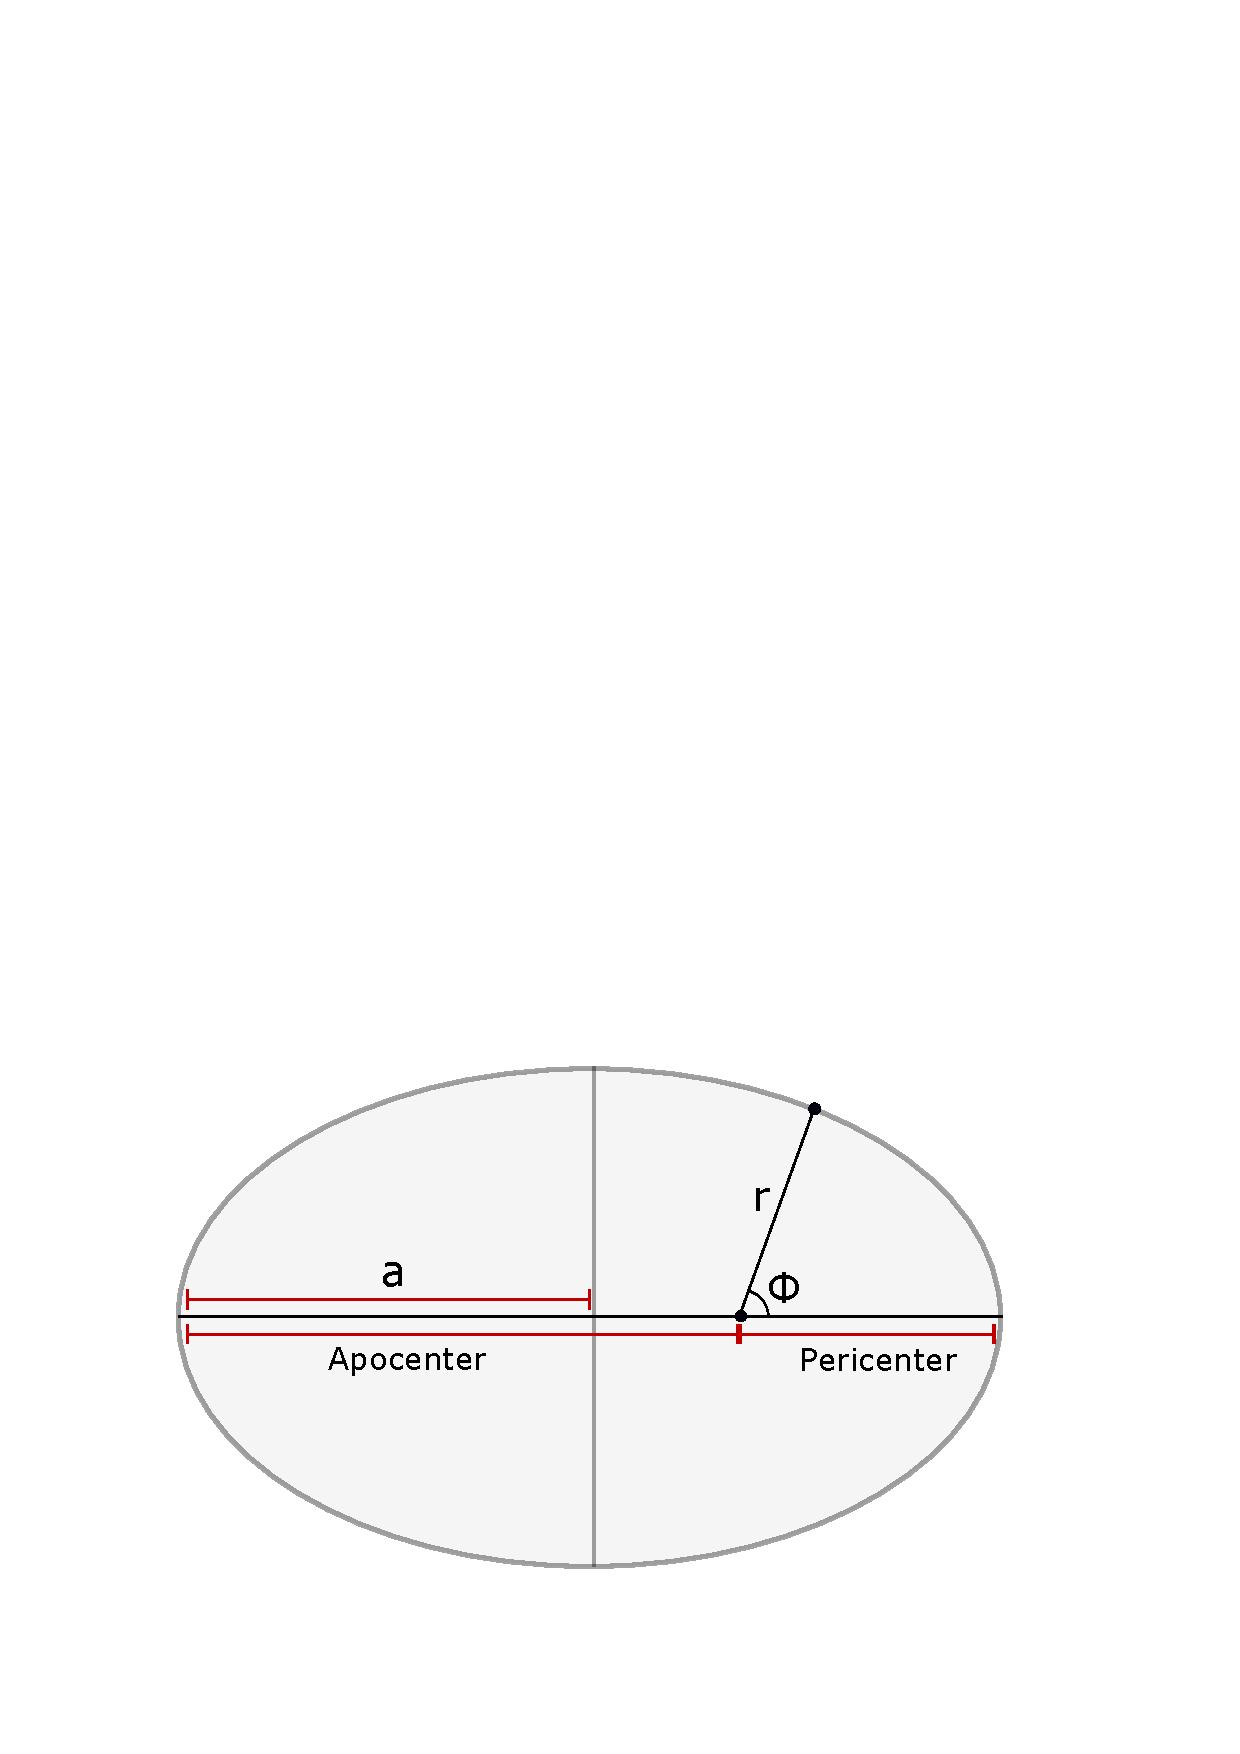
\includegraphics[width=8cm]{../Tesis/Capitulo2/Figures/elipsesencilla.pdf}
\caption{Ellipse}
\label{fig: ellipse}
\end{figure}

\begin{align*}
	&u_1=\frac{1}{a(1-e)}: \text{Pericenter}\\
	&u_2=\frac{1}{a(1+e)}: \text{Apocenter}.
\end{align*}

Expanding the right side of equation (\ref{eq: factorizacion}) and comparing to find that
\begin{subequations}
\begin{align}
	&A = -u_3-Fu_2 -Fu_1\\
	&B = u_2u_3 + u_1u_3 + Fu_1u_2\\
	&C = -u_1u_2u_3.
\end{align}
\end{subequations}

Replacing the pericenter and apocenter and comparing with the coefficients A, B and C given in (\ref{eq: coefficientsFABC}) to find the missing values of $u_3$, $j$ and $g$, gives

\begin{align}
	u_3 = &\left[\kappa - \frac{m}{a}(\gamma+2-2\alpha - \kappa +\alpha)\right]a(1-e^2)\\
	j = &\kappa-1+\frac{m}{a}\left[-(\gamma+2-2\alpha-\kappa+\alpha)\right.\\  \notag
	&\left.+\frac{2}{(1-e^2)}(3\alpha-\beta + 2\gamma\kappa -2\kappa^2 - 4\kappa\alpha + 4\kappa )\right]\\
	g=&\kappa-1-\frac{m}{a}\left(\gamma-\alpha-\kappa+\frac{7}{4}\right).
	\end{align}
	
The equation of motion
\begin{align}
\begin{split}
\label{eq: equationmotionsecond}
	\frac{\ell^2}{GM}\left(\frac{du}{d\phi}\right)^2 = &\left(u-\frac{1}{a(1-e)}\right)\left(u-\frac{1}{a(1+e)}\right)\\
	&\times \left(2\alpha m u-\kappa(2-\kappa)+\frac{m}{a}(\gamma+2-\alpha-\kappa)(1-\kappa)\right.\\
	&\left.+\frac{2\kappa m }{a(1-e^2)}\underbrace{(3\alpha-\beta + 2\gamma\kappa -2\kappa^2 - 4\kappa\alpha + 4\kappa )}_Y\right),
	\end{split}
	\end{align}

replace $j$ to find the angular momentum, 

\begin{align}\label{eq: angularmomentumj+1}
	&\ell^2 = GMa(1-e^2)\left\{\kappa+\frac{m}{a}\left[-(\gamma+2-\alpha-\kappa)+\frac{2Y}{(1-e^2)}\right]\right\},
\end{align}
	
and $g$ to find the energy,
\begin{align} \label{eq: energyg+1}
	\mathcal{H} = - \frac{GM}{2a}\left[\kappa-\frac{m}{a}\left(\gamma-\alpha-\kappa+\frac{7}{4}\right)\right].	
\end{align}
	
Now, considering the conic equation
\begin{align}
	&u(\phi) = \frac{1+e\cos f}{a(1-e^2)}\\
	&f=f(\phi) = \phi - \omega \hspace{0.5cm} \text{(See Figure (\ref{fig: elementosorbitales}))},
\end{align}
where $f$ is the true anomaly and $\omega$ is the longitude of the pericenter.\\


%\begin{figure}[htb!]
%\centering
%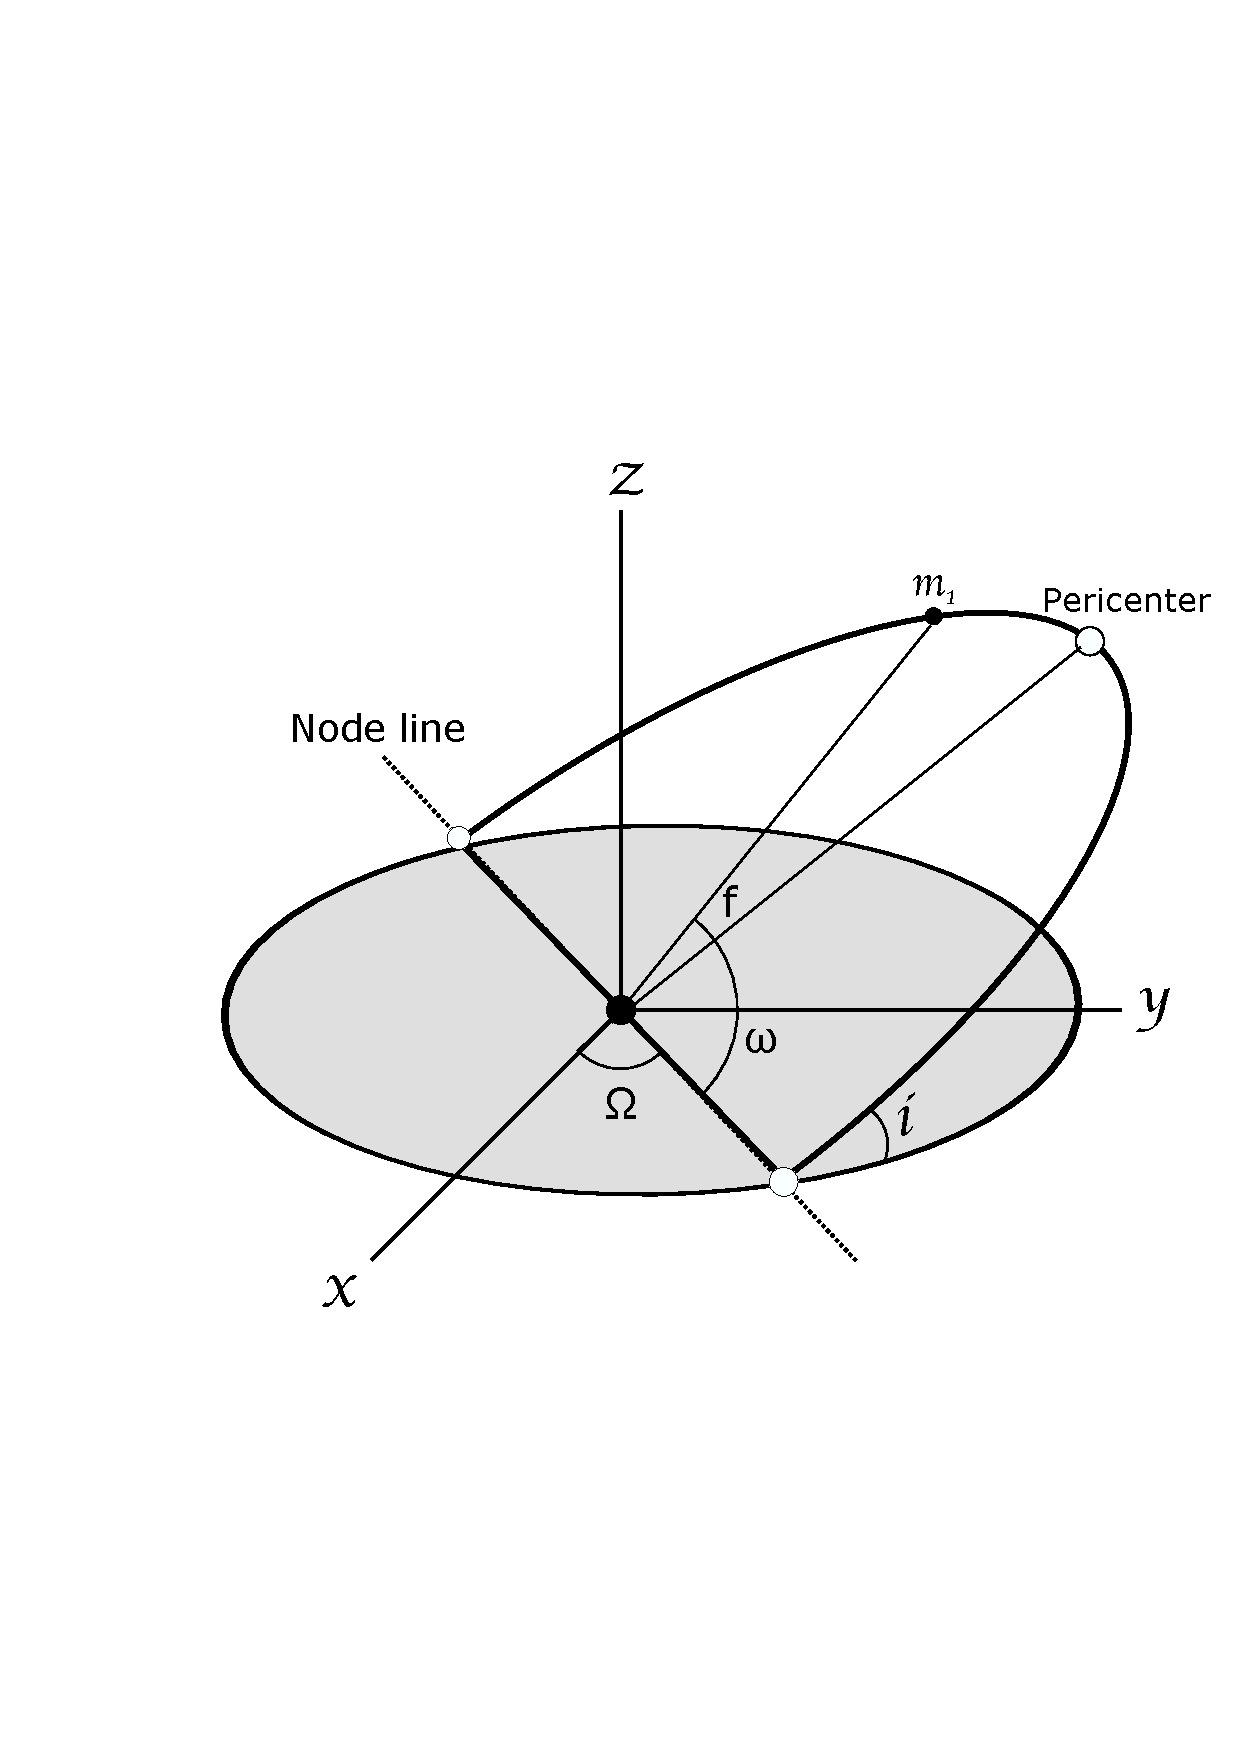
\includegraphics[width=8cm]{../Tesis/Capitulo2/Figures/elementosorbitales.pdf}
%\caption{Configuration of elliptical orbit}
%\label{fig: elementosorbitales}
%\end{figure}

Rewriting the equation (\ref{eq: equationmotionsecond}), where
\begin{align*}
	\frac{du}{d\phi} = -\frac{e\sin f}{a(1-e^2)}\frac{df}{d\phi},
\end{align*}
to obtain
\begin{align}
\label{eq: dfdphi}
\begin{split}
	\frac{df}{d\phi} &=\sqrt{\kappa(2-\kappa)}\left\{1-\frac{m}{a\kappa(2-\kappa)}\left[(1-\kappa)(\gamma+2-\alpha-\kappa)+\frac{\kappa Y}{(1-e^2)}+\frac{\alpha}{1-e^2}\right]\right\}\\
	&\hspace{1.7cm}\times\left[1-\frac{m\alpha e \cos f}{a\kappa (2-\kappa)(1-e^2)}\right].
	\end{split}
\end{align}
All terms inside the curly brackets are constants, so we write
\begin{align}
	\frac{df}{d\phi} =\nu \left[1-\frac{m\alpha e \cos f}{a\kappa (2-\kappa)(1-e^2)}\right],
\end{align}
where 
\begin{align*}
	\nu = \sqrt{\kappa(2-\kappa)}\left\{1-\frac{m}{a\kappa(2-\kappa)}\left[(1-\kappa)(\gamma+2-\alpha-\kappa)+\frac{\kappa Y}{(1-e^2)}+\frac{\alpha}{1-e^2}\right]\right\}
\end{align*}

This can be written as an expansion,
\begin{align*}
	\frac{d(^{(0)}f+^{(2)}f)}{d\phi} =\nu \left[1-\frac{m\alpha e \cos ^{(0)}ff}{a\kappa (2-\kappa)(1-e^2)}\right].
\end{align*}
The zeroth order,
\begin{align*}
	\frac{d^{(0)}f}{d\phi} &=\nu \\
	^{(0)}f &= \nu(\phi-\omega).
\end{align*}
The second order,
\begin{align*}
	\frac{d^{(2)}f}{d\phi}& =-\nu \left[\frac{m\alpha e \cos ^{(0)}f}{a\kappa (2-\kappa)(1-e^2)}\right]  \\
	^{(2)}f & = -\frac{m\alpha e \sin [\nu(\phi-\omega)]}{a\kappa (2-\kappa)(1-e^2)}.
\end{align*}

The true anomaly is
\begin{align}
f =  \nu(\phi-\omega)-\frac{m\alpha e \sin [\nu(\phi-\omega)]}{a\kappa (2-\kappa)(1-e^2)}
\end{align}

To recover the newtonian case we fix the constants as $\gamma = 0$, $\beta = 0$, $\alpha = 0$ y $\kappa = 1$, then
\begin{align*}
f =  \phi-\omega.
\end{align*}

Up to now, there are only differential equations with $\phi$ dependence, but it is possible to recover the time dependence in the equations. From (\ref{eq: angularmomentumthird}) and (\ref{eq: energyg+1}),

\begin{align*}
r^2 d\phi&=\ell\left[1-\frac{\mathcal{H}}{c^2}-\frac{2m}{r}\left(\gamma+\kappa-\alpha\right)\right]dt\\
\end{align*}
and
\begin{align*} 
	\frac{\mathcal{H}}{c^2} &= - \frac{m}{2a}\kappa + \mathcal{O}(\epsilon^4).
\end{align*}

Replacing $\sfrac{\mathcal{H}}{c^2}$ in the expression of $r^2 d\phi$, $\ell$ as given by (\ref{eq: angularmomentumj+1}),

\begin{align}
	&\ell = \sqrt{GMa(1-e^2)\kappa}\left\{1-\frac{m}{2a\kappa}\left[(\gamma+2-\alpha-\kappa)-\frac{2Y}{(1-e^2)}\right]\right\},
\end{align}

and the term $\sqrt{GM\kappa}$ rewritten in terms of the mean anomaly given in (\ref{eq: meanmotion}), the resultant equation is,

\begin{align}
&ndt = \frac{r^2d\phi}{a^2\sqrt{1-e^2}}\left\{1+\frac{2m}{r}(\gamma-\alpha+\kappa)+\frac{m}{2a}\left[(2-\alpha-2\kappa)-\frac{2Y}{1-e^2}\right]+\frac{m}{2a}\left[\alpha\left(1+\frac{\kappa}{2} \right)-\beta\right]\right\}.
\end{align}

From the equation (\ref{eq: dfdphi}), solve for $d\phi$ in terms of $df$ and replace in the equation $ndt$ above. Finally a equation in terms of $df$ and $dt$ is obtained,

\begin{align}
\begin{split}
\frac{df}{dt} =& \frac{na^2\sqrt{1-e^2}\sqrt{\kappa(2-\kappa)}}{r^2}\left\{1-\frac{2m}{r}(\gamma-\alpha+\kappa)-\frac{m}{2a}\left(2-\alpha-2\kappa-\frac{2Y}{1-e^2}\right)\right.\\
&\left.-\frac{m}{a\kappa}\left[\alpha\left(1+\frac{\kappa}{2}\right)-\beta\right]-\frac{\alpha m}{\kappa r (2-\kappa)} \right.\\
&\left.-\frac{m}{2a\kappa (2-\kappa)}\left[(1-\kappa)(\gamma+2-\alpha+\kappa)+\frac{2\kappa Y}{1-e^2}\right].\right\}
	\end{split}
	\end{align}

\subsection{Perturbing Force}

The change of the orbital elements can be determined on account of the perturbative force. It can be identified by comparing with the equation of motion
\begin{align*}
    \mathbf{\ddot{x}}= -\frac{GM}{r^2}\mathbf{x}+\mathbf{F}.
\end{align*}

The perturbative force is $\mathbf{F}$

\begin{align}
\begin{split}
\label{eq: equationofmotion}
\mathbf{F} &=\left\{(1-\kappa) GM+ m\left[2(\beta + \kappa \gamma - \alpha)\frac{GM}{r}-(\gamma+\alpha)\mathbf{\dot{x}}^2+ 3\alpha\frac{\left(\mathbf{x} \cdot \mathbf{\dot{x}}\right)^2}{r^2}\right]\right\}\frac{\mathbf{x}}{r^3}\\
&+\frac{m}{r^3}\left[2(\kappa+\gamma - \alpha)\mathbf{x}\cdot\mathbf{\dot{x}}\right]\mathbf{\dot{x}}+\mathcal{O}(\epsilon^3).
\end{split}
\end{align}

This force can be written as
\begin{align}
\mathbf{F} = \mathcal{R} \mathbf{n}+\mathcal{T}\boldsymbol{\lambda}+\mathcal{W}\mathbf{k}
\end{align}
with
\begin{subequations}
\begin{align}
&\mathbf{n} = \frac{\mathbf{x}}{x}\\
&\boldsymbol{\lambda}  = \frac{d\mathbf{n} }{d\phi} \\
&\mathbf{k}  = \mathbf{n} \times \boldsymbol{\lambda}.
\end{align}
\end{subequations}

Each coefficient is

\begin{align}\label{eq: componetsperturbingforce}
\mathcal{R} = \mathbf{F} \cdot \mathbf{n}, \hspace{0.5cm} \mathcal{T} = \mathbf{F} \cdot \boldsymbol{\lambda}, \hspace{0.5cm}
\mathcal{W} = \mathbf{F} \cdot \mathbf{k}
\end{align}

The radial component is
\begin{subequations}\label{eq: FTWperturbativeforce}
\begin{align}
\begin{split}
	\mathcal{R} &= \frac{n^2a^2}{\kappa r^2}\left\{(1-\kappa)a+m\left[\frac{2a}{r}(\beta-\alpha+2\kappa\gamma + 2\kappa^2)-(2\kappa+\gamma)\kappa \right. \right.\\
	&\left. \left.-(2\gamma+2\kappa+\alpha)a^2\frac{(1-e^2)\kappa}{r^2}+(1-\kappa)\frac{2}{\kappa}\left(\beta-\alpha\left(1+\frac{\kappa}{2}\right)+\frac{\kappa\gamma}{2}\right)\right]\right\},
	\end{split}
\end{align}	
the component ortogonal to $\mathbf{n}$ is
\begin{align}
	\mathcal{T} = 2n^2a^3e\sqrt{\kappa(2-\kappa)}(\kappa+\gamma-\alpha)\frac{m}{r^3}\sin f
\end{align}
and the $\mathbf{k}$ component is
\begin{align}
\mathcal{W} = 0.
\end{align}
\end{subequations}

\subsection{Orbital elements}

The change of the orbital elements in term of the coefficients of the perturbative force are \cite{Brumberg, Larranaga}

\begin{subequations}\label{eq:OsculatingOrbitalElements}
\begin{align}
\frac{da}{dt} &= \frac{2}{n \sqrt{1-e^2}} \left[ e \sin f \mathcal{R} + (1+e\cos f) \mathcal{T} \right] \\
\frac{de}{dt} &= \frac{\sqrt{1-e^2}}{na} \left[ \sin f \mathcal{R} + \frac{2\cos f + e \left( 1 + \cos^2 f \right) }{1 + e\cos f} \mathcal{T} \right] \\
\frac{d \iota}{dt} &= \frac{\sqrt{1-e^2}}{na} \frac{\cos (f+\omega)}{1+e\cos f} \mathcal{W} \\
\frac{d \Omega}{dt} &= \frac{\sqrt{1-e^2}}{na} \frac{\sin (f+\omega)}{(1+e\cos f)\sin \iota } \mathcal{W} \\
\frac{d\omega}{dt} &=\frac{\sqrt{1-e^2}}{nae} \left[ -\cos f \mathcal{R} + \frac{2+e\cos f}{1 + e \cos f} \sin f \mathcal{T} - e  \frac{\sin (f + \omega)}{1 + e \cos f} \cot \iota \mathcal{W} \right].\\
%\frac{dl_0}{dt} &= -\sqrt{1-e^2} \left[ \frac{d\omega}{dt} + \cos \iota \frac{d\Omega}{dt} - \frac{2p}{na^2 (1+e \cos f)} \mathcal{T} \right] ,
\end{align}
\end{subequations}
using the coefficients given in (\ref{eq: FTWperturbativeforce}), we can write
\begin{subequations}
\begin{align}
\frac{da}{dt} &= \frac{2}{n \sqrt{1-e^2}} \left[ e \sin f \mathcal{R} + (1+e\cos f) \mathcal{T} \right] \\
\frac{de}{dt} &= \frac{\sqrt{1-e^2}}{na} \left[ \sin f \mathcal{R} + \frac{2\cos f + e \left( 1 + \cos^2 f \right) }{1 + e\cos f} \mathcal{T} \right] \\
\frac{d \iota}{dt} &= 0 \\
\frac{d \Omega}{dt} &= 0 \\
\frac{d\omega}{dt} &=\frac{\sqrt{1-e^2}}{nae} \left[ -\cos f \mathcal{R} + \frac{2+e\cos f}{1 + e \cos f} \sin f \mathcal{T}  \right], \\
%\frac{dl_0}{dt} &= \sqrt{1-e^2} \left[\frac{2p}{na^2 (1+e \cos f)} \mathcal{T} \right] ,
\end{align}
\end{subequations}

where $p$ the \textit{semi-latus rectum}
\begin{align}
 r = \frac{p}{1+e\cos f} = \frac{a(1-e^2)}{1+e\cos f}.
\end{align}


Up to this approximative order, the perturbative force $\mathbf{F}$ does not have a component in the $\mathbf{k}$ direction. 

	
	
%Eliminate all terms $h_{0i}$ acorde to (\ref{eq:gmetricppn}).
%\begin{align*}
%\begin{split}
%\ddot{x}^j &= \frac{1}{2}c^2\partial_{j}^{(2)}h_{00}+\frac{1}{2}c^2\partial_{j}^{(4)}h_{00}-\frac{1}{2}c^{2(2)}h_{jk}\partial_{k}^{(2)}h_{00} -\frac{1}{2}c\dot{x}^j\partial_0^{(2)}h_{00} \\
%&-c\dot{x}^k\partial_0^{(2)}h_{jk}
%-\dot{x}^j\dot{x}^k\partial_k^{(2)}h_{00} - \left(\partial_k^{(2)}h_{jl}-\frac{1}{2}\partial_j^{(2)}h_{kl}\right)\dot{x}^k\dot{x}^l + \mathcal{O}(\epsilon^3)
%\end{split}
%\end{align*}



%\begin{align*}
%\ddot{x}^j &= \frac{1}{2}c^2\partial_{j}\left(\frac{2\kappa m}{r}\right) + \frac{1}{2}c^2\partial_{j}\left(\frac{2(\alpha-\beta)m^2}{r^2}\right)-\frac{1}{2}c^{2} \left[\frac{2m}{r}\left((\gamma-\alpha)\delta_{jk}+\alpha\frac{x_j x_k}{r^2}\right)\right]\partial_{k}\left(\frac{2\kappa m}{r}\right)\\
%&-\frac{1}{2}c\dot{x}^j\partial_0\left(\frac{2\kappa m}{r}\right)-c\dot{x}^k\partial_0\left[\frac{2m}{r}\left((\gamma-\alpha)\delta_{jk}+\alpha\frac{x_j x_k}{r^2}\right)\right]-\dot{x}^j\dot{x}^k\partial_k\left(\frac{2\kappa m}{r}\right)\\
%&\left(\partial_k\left[\frac{2m}{r}\left((\gamma-\alpha)\delta_{jl}+\alpha\frac{x_j x_l}{r^2}\right)\right]-\frac{1}{2}\partial_j\left[\frac{2m}{r}\left((\gamma-\alpha)\delta_{kl}+\alpha\frac{x_k x_l}{r^2}\right)\right]\right)\dot{x}^k\dot{x}^l+ \mathcal{O}(\epsilon^3)
%\end{align*}


 




